Es  werden nun  anhand  der  Phasengangmethode sowohl  ein  PI-  wie auch  ein
PID-Regler f\"ur die in Abschnitt~\ref{subs:frequenzgang} ausgemessene Strecke
dimensioniert (siehe n\"achster Abschnitt f\"ur PID-Regler).

Tabelle~\ref{tab:terms}  fasst  die  h\"aufig verwendeten  Begriffe  in  einer
\"Ubersicht zusammen:

\begin{longtable}{lp{60mm}}
    \toprule
    \endhead
    \endfoot
    \endlastfoot

    % CONTENT HERE ---------------------------------------------------------- %

    $H_s(j\omega)                                                                   $ &  \"Ubertragungsfunktion der Regelstrecke \\
    $A_s(j\omega)=|H_s(j\omega)|                                                    $ &  Amplitudengang der Regelstrecke \\
    $\varphi_s(j\omega)=arg(H_s(j\omega))                                           $ &  Phasengang der Regelstrecke \\
    $H_r(j\omega)                                                                   $ &  \"Ubertragungsfunktion des Reglers \\
    $A_r(j\omega)=|H_r(j\omega)|                                                    $ &  Amplitudengang des Reglers \\
    $\varphi_r(j\omega)=arg(H_r(j\omega))                                           $ &  Phasengang des Reglers \\
    $H_o(j\omega)=H_s \cdot H_r(j\omega)                                            $ &  \"Ubertragungsfunktion des offenen Regelkreises \\
    $A_o(j\omega)=|H_o(j\omega)|                                                    $ &  Amplitudengang des offenen Regelkreises \\
    $\varphi_o(j\omega)=arg(H_o(j\omega))=\varphi_s(j\omega)+\varphi_r(j\omega)     $ &  Phasengang des offenen Regelkreises \\
    $H_{rpid}= K_{rk}\Big[ \frac{(1+sT_{nk})(1+sT_{vk})}{sT_{nk}}\Big]              $ & \"Ubertragungsfunktion des PID-Reglers \\
    $H_{rpi} = K_{rk}\Big[ 1 + \frac{1}{sT_{nk}} \Big]                              $ & \"Ubertragungsfunktion des PI-Reglers \\

    \bottomrule
    \caption{Die wichtigsten Begriffsdefinitionen}
    \label{tab:terms}
\end{longtable}


% ---------------------------------------------------------------------------- %
\subsubsection*{Ziel}
% ---------------------------------------------------------------------------- %
Das  Ziel dieses  Abschnittes ist  die Bestimmung  der Parameter  $K_{rk}$ und
$T_{nk}$ in der \"Ubertragungsfunktion des Reglers:

\begin{equation} \label{eq:pi:target}
    H_{rpi} = K_{rk} \cdot \biggl[ 1 + \frac{1}{s \cdot T_{nk}} \biggr]
\end{equation}


% ---------------------------------------------------------------------------- %
\subsubsection{Bestimmung der Reglerfrequenz $\mathbf{\boldsymbol{\omega}_{pi}}$}
% ---------------------------------------------------------------------------- %

Zuerst  wird im  Phasengang der  Strecke gem\"ass  Gleichung~\ref{eq:pi:phi_s}
die     Frequenz     $\omega_{pi}$      bestimmt,     f\"ur     welche     die
Phase     der    Strecke     $-90\degree$     betr\"agt,    ersichtlich     in
Abbildung~\ref{fig:pi:omega_pi}\footnotemark[4].

\begin{equation} \label{eq:pi:phi_s}
    \varphi_s(\omega_{pi}) = -90 \degree
\end{equation}

\footnotetext[4]{%
    Der  Winkel  stellt  keinen   endg\"ultigen  Wert  dar. Dieser  wurde  von
    Jakob  Zellweger  fixiert, um  eine  graphische  Evaluation \"uberhaupt  zu
    erm\"oglichen. Durch Anpassung dieses Wertes kann je nach Regelstrecke das
    Regelverhalten weiter optimiert werden.
}

\begin{figure}[h! width=\pagewidth]
    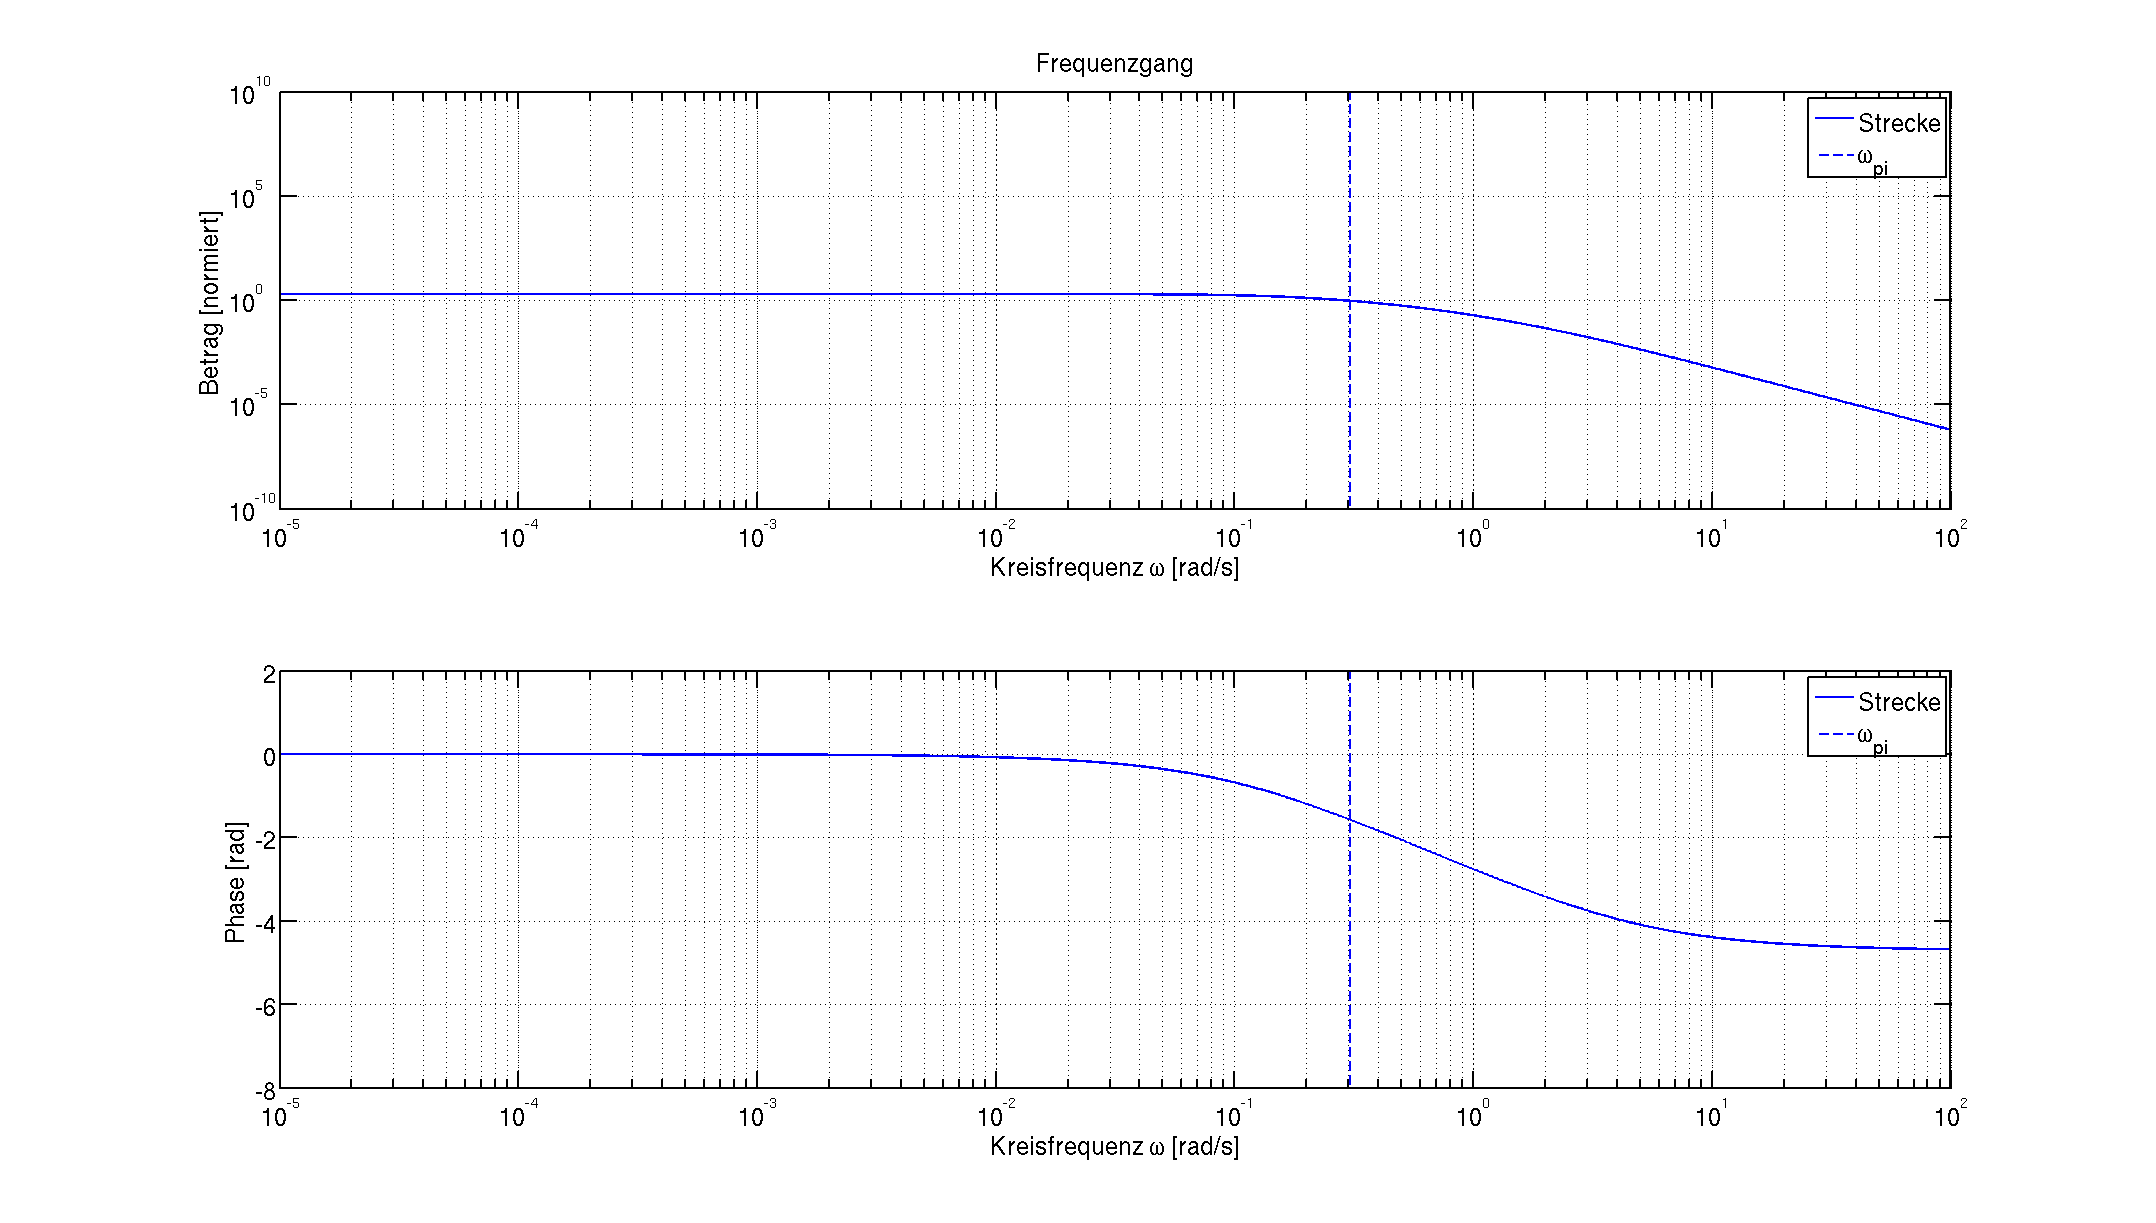
\includegraphics[width=\textwidth]{images/piStreckeOmegaPI.png}
    \caption{%
        Amplituden- und  Phasengang der Strecke mit  $\omega_{pi}$ eingetragen
        (vertikale gestrichelte Linie).
    }
    \label{fig:pi:omega_pi}
\end{figure}

Wie    man   aus    Abbildung~\ref{fig:pi:omega_pi}   ablesen    kann,   liegt
dieser   Wert  f\"ur   $\omega_{pi}$  in   unserem  Beispiel   bei  ungef\"ahr
$\SI{0.3}{\per\second}$. Die Kontrollrechnung mittels Matlab ergibt:

\begin{equation} \label{eq:pi:omega_pi}
    \omega_{pi} = \SI{0.3039}{\per\second}
\end{equation}


% ---------------------------------------------------------------------------- %
\subsubsection{Bestimmung von $\mathbf{T_{nk}}$}
% ---------------------------------------------------------------------------- %
Damit kann nun $T_{nk}$ direkt berechnet werden\footnotemark[5]:

\begin{equation} \label{eq:pi:omega_pi}
    T_{nk} = \frac{1}{\omega_{pi}} = \frac{1}{\SI{0.3039}{\per\second}} = \SI{3.2902}{\second}
\end{equation}

\footnotetext[5]{%
    Um die  Akkumulation von Ungenauigkeiten  zu minimieren, werden bei diesen
    Berechnungen  die  genauen  Werte  aus  Matlab  verwendet  und  nicht  die
    gerundeten  Zwischenresultate,  was  zu   Abweichungen  zu  den  von  Hand
    berechneten Ergebnissen f\"uhren kann.
}


% ---------------------------------------------------------------------------- %
\subsubsection{Bestimmung der Durchtrittsfrequenz $\mathbf{\boldsymbol{\omega}_d}$}
% ---------------------------------------------------------------------------- %

Die   Durchtrittsfrequenz  ist   die   Frequenz,  bei   der  die   betrachtete
\"Ubertragungsfunktion $H(j\omega)$ eine Verst\"arkung von $\SI{0}{\decibel} =
1$  aufweist. In der  Phasengangmethode soll  sie so  festgelegt werden,  dass
der  offene  Regelkreis  Gleichung~\ref{eq:phi_o} erf\"ullt. Dabei  ist  f\"ur
$\varphi_s$, abh\"angig vom gew\"unschten \"Uberschwingverhalten, ein Wert aus
Tabelle~\ref{tab:phi_s} auszuw\"ahlen\footnotemark[6].  Nach dem Festlegen der
Durchtrittsfrequenz (in  unserem Beispiel werden wir  $16.3\%$ anstreben) wird
dann im n\"achsten Abschnitt die Verst\"arkung des Reglers noch angepasst.

\footnotetext[6]{%
    Die  Werte f\"ur  $\varphi_s$  aus  Tabelle~\ref{tab:phi_s} stellen  keine
    abschliessende  Auflistung dar  und  sind lediglich  als Anhaltspunkte  zu
    betrachten. Weicht das Verhalten des geschlossenen Regelkreises am Schluss
    zu stark  vom gew\"unschten  Ergebnis ab, besteht  durch die  Wahl anderer
    Werte f\"ur $\varphi_s$ die M\"oglichkeit weiterer Optimierung.
}

\begin{equation} \label{eq:phi_o}
    \varphi_o(\omega_d)=\varphi_s.
\end{equation}

\clearpage

\begin{longtable}{llll}
    \toprule
    \endhead
    \endfoot
    \endlastfoot

    % CONTENT HERE ---------------------------------------------------------- %

    \"Uberschwingen & 0\%              & 16.3\%           & 23.3\% \\
    $\varphi_s$        & $-103.7 \degree$ & $-128.5 \degree$ & $-135 \degree$ \\

    \bottomrule
    \caption{Werte f\"ur $\varphi_s$}
    \label{tab:phi_s}
\end{longtable}

Um    Gleichung~\ref{eq:phi_o}    auswerten     zu    k\"onnen,    wird    der
Phasengang   des   offenen   Regelkreises   ben\"otigt. Dazu   wird   der   in
Gleichung~\ref{eq:pi:omega_pi}    erhaltene    Wert    f\"ur    $T_{nk}$    in
die   \"Ubertragungsfunktion    des   Reglers   (Gleichung~\ref{eq:pi:target})
eingesetzt. $K_{rk}$  ist  noch  unbekannt,  hat aber  auf  die  Phase  keinen
Einfluss und wird somit vorerst einfach auf 1 gesetzt.

\begin{gather} \label{eq:pi:target:inserted}
    \begin{split}
        H_{rpi} & = K_{rk} \cdot \biggl[ 1 + \frac{1}{s \cdot T_{nk}} \biggr] \\
                & = 1      \cdot \biggl[ 1 + \frac{1}{s \cdot \SI{3.2902}{\second}} \biggr]
    \end{split}
\end{gather}

Daraus kann nun der Frequenzgang  $H_o$ des offenen Regelkreises identifiziert
werden.

\begin{gather} \label{eq:pi:h_open}
    \begin{split}
        H_o (s) & = H_{rpi} (s) \cdot H_s (s) \\
            & = \Biggl(
                    K_{rk} \cdot \biggl[ 1 + \frac{1}{s \cdot T_{nk}} \biggr]
                \Biggr)
                \cdot
                K_s
                \cdot
                \Biggl(
                        \frac{1}{1 + s \cdot T_1}
                  \cdot \frac{1}{1 + s \cdot T_2}
                  \cdot \frac{1}{1 + s \cdot T_2}
                \Biggr) \\
            & = \Biggl(
                    1 \cdot \biggl[ 1 + \frac{1}{s \cdot \SI{3.2902}{\second}} \biggr]
                \Biggr)
                \cdot
                2
                \cdot
                \Biggl(
                          \frac{1}{1 + s \cdot \SI{0.4134}{\second}}
                    \cdot \frac{1}{1 + s \cdot \SI{1.4894}{\second}}
                    \cdot \frac{1}{1 + s \cdot \SI{5.3655}{\second}}
                \Biggr)
    \end{split}
\end{gather}


Von   besonderem    Interesse   ist   der    Phasengang   $\varphi_o(j\omega)$
dieser   \"Ubertragungsfunktion. Wie  oben   festgelegt,  soll   ein  maximals
\"Uberschwingen  von   ca. $16.3\%$  angestrebt  werden. Dazu   muss  gem\"ass
Tabelle~\ref{tab:phi_s}  die Durchtrittsfrequenz  $\omega_d$ gefunden  werden,
an  welcher der  offene  Regelkreis eine  Phase  von $-128.5\degree$  aufweist
(Gleichung~\ref{eq:phi_o}). In   Abbildung~\ref{fig:pi:omega_d}   kann   diese
Beziehung graphisch verifiziert werden.

\begin{figure}[h! width=\pagewidth]
    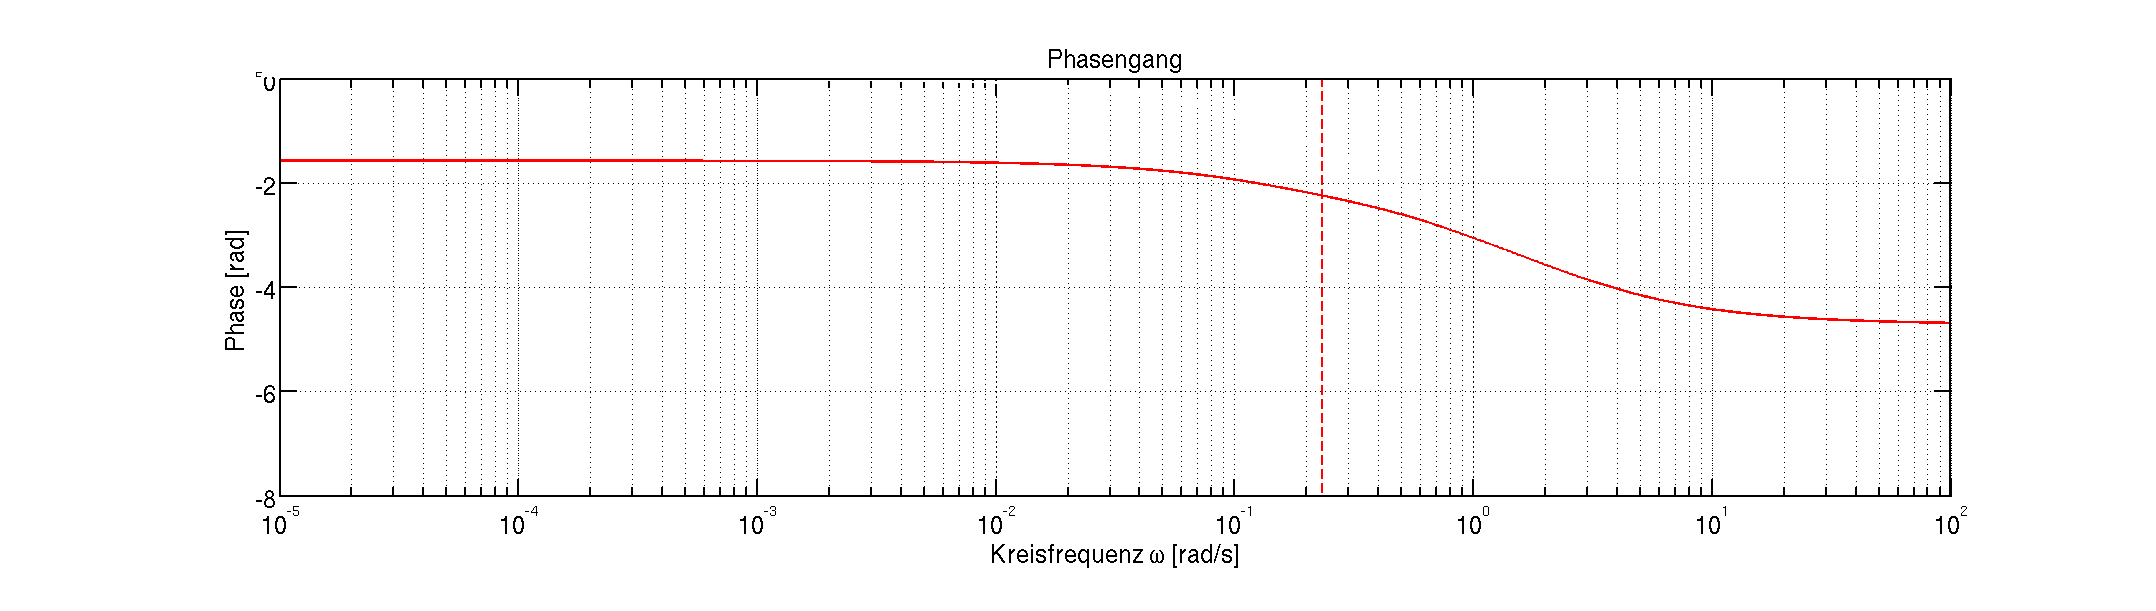
\includegraphics[width=\textwidth]{images/piOffenerRegelkreisPhasengang.png}
    \caption{%
        Phasengang   $\varphi_o(j\omega)$   des   offenen   Regelkreises   mit
        eingetragener Durchtrittsfrequenz $\omega_{d}$ (vertikale gestrichelte
        Linie). Wie man  sieht, weist der offene  Regelkreis unseres Beispiels
        bei dieser Kreisfrequenz eine Phase von $-128.5\degree$ auf
        (etwa $\SI{-2.24}{\radian}$).
    }
    \label{fig:pi:omega_d}
\end{figure}

Dies ergibt f\"ur die Durchtrittsfrequenz:
\begin{equation} \label{eq:pi:omega_d}
    \omega_d = \SI{0.2329}{\per\second}
\end{equation}


% ---------------------------------------------------------------------------- %
\subsubsection{Bestimmung der Reglerverst\"arkung $\mathbf{K_{rk}}$}
% ---------------------------------------------------------------------------- %

Im  letzten  Schritt  muss  nun, wie im  vorherigen  Abschnitt  erw\"ahnt, die
Verst\"arkung  $K_{rk}$   des  Reglers   noch  angepasst  werden,   damit  der
offene   Regelkreis  bei   der  angestrebten   Durchtrittsfrequenz  $\omega_d$
auch  effektiv  eine Verst\"arkung  von  1  aufweist.  Dazu  wird  $j\omega_d$
in  Gleichung~\ref{eq:pi:h_open}  f\"ur  den   Parameter  $s$  eingesetzt  und
$|H_o(j\omega_d)| = 1$ gesetzt.

\begin{gather} \label{eq:pi:A_o_set_to_one}
    \begin{split}
        A_o & = | H_o (j\omega_d) | = | H_{rpi} (j\omega) \cdot H_s (j\omega)| \\
            & = \abs*{
                    \bigg(
                        K_{rk} \cdot \biggl[ 1 + \frac{1}{j \cdot \omega_d \cdot T_{nk}} \biggr]
                    \bigg)
                    \cdot
                    K_s
                    \cdot
                    \bigg(
                            \frac{1}{1 + j \cdot \omega_d \cdot T_1}
                      \cdot \frac{1}{1 + j \cdot \omega_d \cdot T_2}
                      \cdot \frac{1}{1 + j \cdot \omega_d \cdot T_2}
                      \bigg)} \\
              & = 1
    \end{split}
\end{gather}

Mit den Werten
\begin{equation} \label{eq:pi:values}
    \begin{split}
        K_s      & = 2                    \\
        T_{nk}   & = \SI{3.2902}{\second} \\
        T_1      & = \SI{0.4134}{\second} \\
        T_2      & = \SI{1.4894}{\second} \\
        T_3      & = \SI{5.3655}{\second} \\
        \omega_d & = \SI{0.2329}{\radian\per\second}
    \end{split}
\end{equation}

l\"ost  man Gleichung  \ref{eq:pi:A_o_set_to_one}  nun nach  $K_{rk}$ auf  und
erh\"alt:

\begin{equation} \label{eq:pi:k_rk_result}
    K_{rk} = 0.517577
\end{equation}


\clearpage
% ---------------------------------------------------------------------------- %
\subsubsection{Resultat}
% ---------------------------------------------------------------------------- %

Somit ist der PI-Regler vollst\"andig bestimmt und hat folgende Form:

\begin{equation} \label{eq:pi:result}
    H_{rpi} = 0.518 \cdot \biggl[ 1 + \frac{1}{s \cdot \SI{3.29}{\second}} \biggr]
\end{equation}

In Abbildung~\ref{fig:pi:all} sind die  wichtigsten Werte f\"ur diesen Prozess
nochmals in einer \"Ubersicht zusammengefasst.

\begin{figure}[h! width=\pagewidth]
    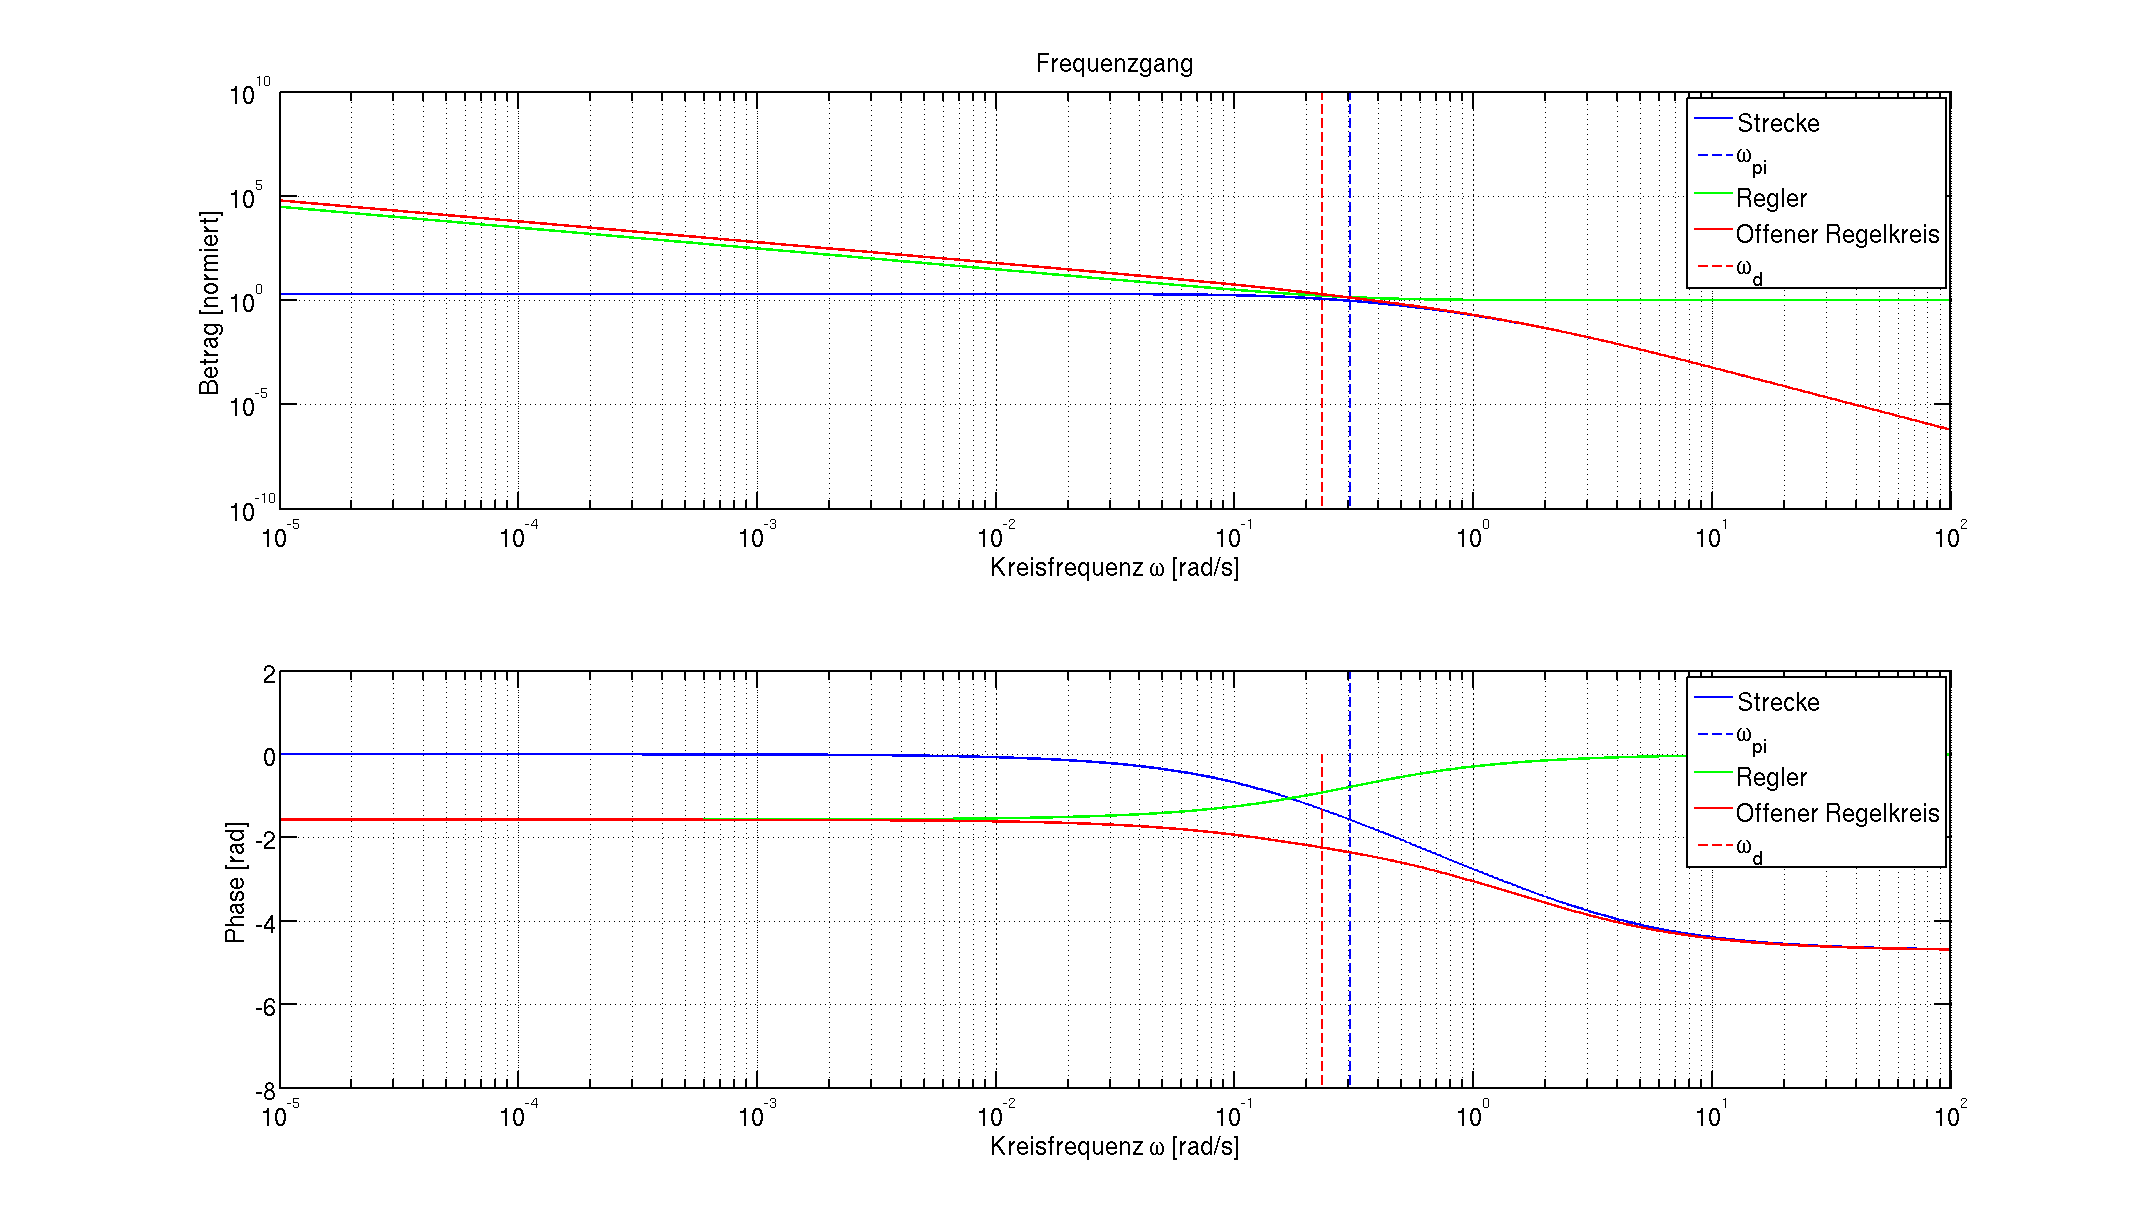
\includegraphics[width=\textwidth]{images/piBode.png}
    \caption{%
        Frequenzgang des Reglers (gr\"un), der  Strecke (blau) und des offenen
        Regelkreises (rot).
    }
    \label{fig:pi:all}
\end{figure}
